\documentclass{scrartcl}

\usepackage[utf8]{inputenc}
\usepackage[T1]{fontenc}
\usepackage{lmodern}
\usepackage{babel}
\usepackage{amsmath}
\usepackage{amsthm}
\usepackage{mathtools}
\usepackage[dvipsnames]{xcolor}
\usepackage{tikz}

\usepackage[
backend=biber,
% style=alphabetic,
sorting=none
]{biblatex}

\addbibresource{whitepaper.bib}

\title{Rule based Symbolic Reasoning}
\author{Matthias Lochbrunner}
\date{\today}

\theoremstyle{definition}
\newtheorem{exmp}{Example}[section]

\begin{document}
\maketitle
\begin{center}
	\textbf{Abstract}
\end{center}
\begin{abstract}
	The combination of a rule based beam search and with deep learning is a promising approach to solve mathematical problems.
	One obstacle to overcome is the amount of possible branches in that search when the number of rules and depth of the calculation increases.
	This paper proposes this issue by constantly shrinking the beam size a multi-head neuronal network:
	A policy head to select rules and positions in the current term. A value head to evaluate the probability that this trace might lead to desired solution.
	Both heads help to reduce the beam size such that solving advanced mathematical problems is feasible.
\end{abstract}

\section{Motivation}

As current approaches to solve mathematical problems are using a complex but fixed rule set, it takes manual effort to increase their capabilities. [Citation needed]
The here described generic approach could be capable to absorb additional formal described rules without the need of manual work.
Furthermore it is not limited to mathematical calculus as long as the domain can be described by a well defined human readable rules.
The correctness of the result only depends on the correctness of the given rules.

\section{Method}

Given a problem, e.g. solve a equation $T_1\left(x\right)\equiv T_2\left(x\right)$ for $x$ the beam search could try to apply various rules at different nodes at the syntax tree of the equation.
The policy head proposes the most promising combination of rules and positions in the current equation.
The accumulated outcome of the value head can cancel the attempt solution path as it "seems" unlikely the this attempt may succeed.

\subsection{Apply a Rule}

Every rule has the shape of $A \Longrightarrow B$ or $A \equiv B$ which is equivalent to $A \Longleftrightarrow B$ or just the combination of $A \Longrightarrow B$ and $B \Longrightarrow A$.
Without loss of correctness we just use the first shape $A \Longrightarrow B$ in this paper. Given the term $T\left(x\right)$ with the depth $d$ of the corresponding syntax tree representation.
We try to match condition $A$ with any position $p \in \big\{ n_1, n_2, \dots, n_k \forall k \leq d, \forall n_i \leq s^i \big\}$ of term $T\left(x\right)$ where $s$ is the maximal number of children per node the syntax tree.
Doing so results in a list of possible positions $p_j$ with the required substitution table $M_j: S_c \to S_t$ where $S_t$ is a subset of the symbols in term $T$ and $S_c$ a subset of the symbols in the condition $A$.
Lets name the sub-terms of $T_{n_1, n_2, \dots, n_d}$ where $T_1$ for instance is the first child node of the root in that tree.
$T_{1,1}$ the first child of $T_1$ and so on.
Then the application of that rule results new terms $T^{(j)}$ where the nodes at $p_j$ get replaced by $B'^{M_j}$ which is $B$ with symbols mapped by $M_j$. 

\begin{exmp}
Application of the derivative rule for polynomials

Consider the derivative rule
\begin{align}
	\frac{\partial}{\partial {\color{red}x}} {\color{red}x}^{\color{blue}n} \Longrightarrow n\cdot {\color{red}x}^{{\color{blue}n}-1} 
\end{align}
applied to the term
\begin{align}
	\frac{\partial}{\partial {\color{red}z}} {\color{red}z}^4 
\end{align}.
Using the symbolic mapping ${\color{red}x \coloneqq z}$ and ${\color{blue}n \coloneqq {\color{blue}4}}$ leads to the new term
\begin{align}
	{\color{blue}4}\cdot {\color{red}z}^{{\color{blue}4}-1} 
\end{align}.

\end{exmp}

\subsection{Policy and Value Heads}

Based on two different architecture multi-head heads for value and policy estimation \cite{44806}.

The policy head suggests useful locations and rules to apply on the given term. This outcome is used to shrink the width of the search beam.
It turned out that it is very important to suppress non-sense rule application as they can blow up the beam. (Negative training samples.)

The value head estimates how likely the given term might lead to success. If the value is below a specified threshold the calculation-track gets cancelled.

\subsubsection{Challenges for Tree Structured Data}
As each term is represented as directed acyclic graph standard neuronal operation can not be applied on this input.
The CNN based network uses an adapted operation for tree structured data.
Special positional encoding for transformer based architecture.

\begin{figure}[!htbp]
	\centering
	
% sample id: #19818
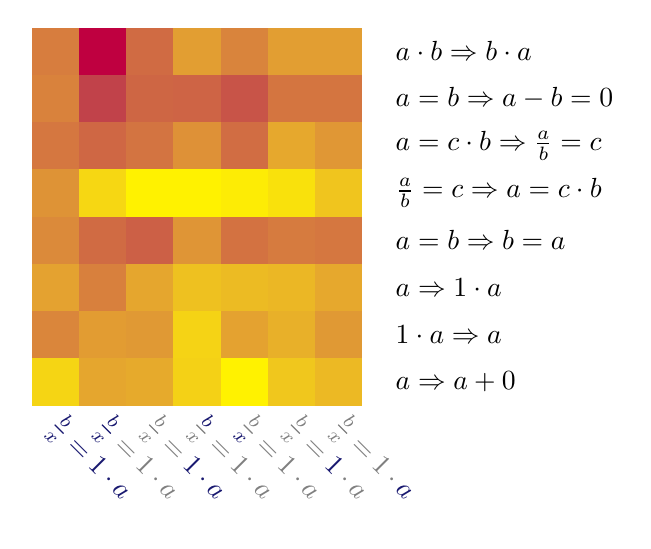
\begin{tikzpicture}[scale=0.6]
    \foreach \y [count=\p] in {
        {40,0,30,58,44,58,58},
        {43,6,27,26,17,36,36},
        {37,28,35,51,31,63,54},
        {52,87,100,100,97,92,78},
        {47,30,24,53,34,39,37},
        {60,42,62,76,73,71,63},
        {45,57,55,85,60,67,55},
        {86,62,64,84,100,79,72},
        } {
        \foreach \x [count=\r] in \y {
            \node[fill=yellow!\x!purple, minimum size=6mm, text=white] at (\r,-\p) {};
        }
    }
    \foreach \t [count=\p] in {
        $a\cdot b \Rightarrow b\cdot a $,
        $a=b \Rightarrow a-b=0 $,
        $a=c\cdot b \Rightarrow \frac{a}{b}=c $,
        $\frac{a}{b}=c \Rightarrow a=c\cdot b $,
        $a=b \Rightarrow b=a $,
        $a \Rightarrow 1\cdot a $,
        $1\cdot a \Rightarrow a $,
        $a \Rightarrow a+0 $
    } {
        \node[anchor=west] at (8, -\p) {\t};
    }
    \foreach \t [count=\r] in {
        $\textcolor{MidnightBlue}{\frac{b}{x}=1\cdot a}$,
        $\textcolor{Gray}{\textcolor{MidnightBlue}{\frac{b}{x}}=1\cdot a}$,
        $\textcolor{Gray}{\frac{b}{x}=\textcolor{MidnightBlue}{1\cdot a}}$,
        $\textcolor{Gray}{\frac{\textcolor{MidnightBlue}{b}}{x}=1\cdot a}$,
        $\textcolor{Gray}{\frac{b}{\textcolor{MidnightBlue}{x}}=1\cdot a}$,
        $\textcolor{Gray}{\frac{b}{x}=\textcolor{MidnightBlue}{1}\cdot a}$,
        $\textcolor{Gray}{\frac{b}{x}=1\cdot \textcolor{MidnightBlue}{a}}$
    } {
        \node[anchor=west, rotate=-45] at (\r - 0.2, -8.7) {\t};
    }
    \end{tikzpicture}
    
	\caption{Policy Network output: Each row is a possible rule. Each column a position in the initial term. Impossible rule applications are filtered out here.} \label{fig:M1}
\end{figure}

\subsection{Data loop}

From given (training) problems the algorithm trains itself by the three-T-loop: 

\begin{itemize}
	\item \textbf{Try} to solve some of the training problems.
	\item \textbf{Trace} the calculation steps of the solved problems and create training samples out of them.
	\item \textbf{Train} the model with these useful and useless trainings steps created.
\end{itemize}

\section{Results}
We have defined all basic rules to perform the given problems as scenario configuration.

\begin{figure}[!htbp]
	\centering
	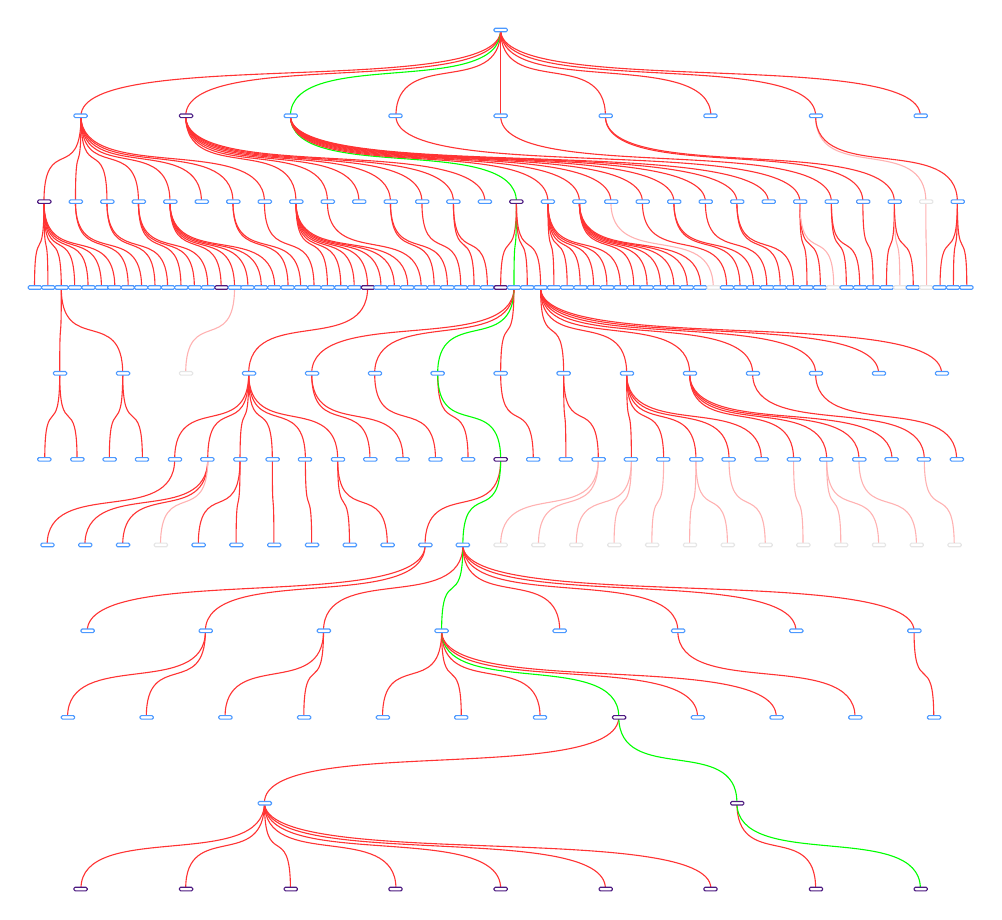
\begin{tikzpicture}[every node/.style={rectangle,fill=white,rounded corners=0.451}]
	\tikzset{xcolor/.code args={#1=#2}{
		\definecolor{mytemp}{rgb}{#2}
		\tikzset{draw=mytemp}
		}
	}
	\fontsize{0.5634}{0.6761}\selectfont
	\draw[draw=red!80] (-5.33,4.36) .. controls (-5.33,5.24) and (0.00,4.58) .. (0.00,5.45);
	\draw[draw=red!80] (-5.80,3.27) .. controls (-5.80,4.15) and (-5.33,3.49) .. (-5.33,4.36);
	\draw[draw=red!80] (-5.92,2.18) .. controls (-5.92,3.05) and (-5.80,2.40) .. (-5.80,3.27);
	\draw[draw=red!80] (-5.75,2.18) .. controls (-5.75,3.05) and (-5.80,2.40) .. (-5.80,3.27);
	\draw[draw=red!80] (-5.58,2.18) .. controls (-5.58,3.05) and (-5.80,2.40) .. (-5.80,3.27);
	\draw[draw=red!80] (-5.60,1.09) .. controls (-5.60,1.96) and (-5.58,1.31) .. (-5.58,2.18);
	\draw[draw=red!80] (-5.79,-8.88e-16) .. controls (-5.79,0.873) and (-5.60,0.218) .. (-5.60,1.09);
	\draw[draw=red!80] (-5.38,-8.88e-16) .. controls (-5.38,0.873) and (-5.60,0.218) .. (-5.60,1.09);
	\draw[draw=red!80] (-4.80,1.09) .. controls (-4.80,1.96) and (-5.58,1.31) .. (-5.58,2.18);
	\draw[draw=red!80] (-4.97,-8.88e-16) .. controls (-4.97,0.873) and (-4.80,0.218) .. (-4.80,1.09);
	\draw[draw=red!80] (-4.55,-8.88e-16) .. controls (-4.55,0.873) and (-4.80,0.218) .. (-4.80,1.09);
	\draw[draw=red!80] (-5.41,2.18) .. controls (-5.41,3.05) and (-5.80,2.40) .. (-5.80,3.27);
	\draw[draw=red!80] (-5.24,2.18) .. controls (-5.24,3.05) and (-5.80,2.40) .. (-5.80,3.27);
	\draw[draw=red!80] (-5.07,2.18) .. controls (-5.07,3.05) and (-5.80,2.40) .. (-5.80,3.27);
	\draw[draw=red!80] (-4.90,2.18) .. controls (-4.90,3.05) and (-5.80,2.40) .. (-5.80,3.27);
	\draw[draw=red!80] (-5.40,3.27) .. controls (-5.40,4.15) and (-5.33,3.49) .. (-5.33,4.36);
	\draw[draw=red!80] (-4.73,2.18) .. controls (-4.73,3.05) and (-5.40,2.40) .. (-5.40,3.27);
	\draw[draw=red!80] (-4.56,2.18) .. controls (-4.56,3.05) and (-5.40,2.40) .. (-5.40,3.27);
	\draw[draw=red!80] (-5.00,3.27) .. controls (-5.00,4.15) and (-5.33,3.49) .. (-5.33,4.36);
	\draw[draw=red!80] (-4.39,2.18) .. controls (-4.39,3.05) and (-5.00,2.40) .. (-5.00,3.27);
	\draw[draw=red!80] (-4.23,2.18) .. controls (-4.23,3.05) and (-5.00,2.40) .. (-5.00,3.27);
	\draw[draw=red!80] (-4.60,3.27) .. controls (-4.60,4.15) and (-5.33,3.49) .. (-5.33,4.36);
	\draw[draw=red!80] (-4.06,2.18) .. controls (-4.06,3.05) and (-4.60,2.40) .. (-4.60,3.27);
	\draw[draw=red!80] (-3.89,2.18) .. controls (-3.89,3.05) and (-4.60,2.40) .. (-4.60,3.27);
	\draw[draw=red!80] (-3.72,2.18) .. controls (-3.72,3.05) and (-4.60,2.40) .. (-4.60,3.27);
	\draw[draw=red!80] (-4.20,3.27) .. controls (-4.20,4.15) and (-5.33,3.49) .. (-5.33,4.36);
	\draw[draw=red!80] (-3.55,2.18) .. controls (-3.55,3.05) and (-4.20,2.40) .. (-4.20,3.27);
	\draw[draw=red!80] (-3.38,2.18) .. controls (-3.38,3.05) and (-4.20,2.40) .. (-4.20,3.27);
	\draw[draw=red!30] (-4.00,1.09) .. controls (-4.00,1.96) and (-3.38,1.31) .. (-3.38,2.18);
	\draw[draw=red!80] (-3.21,2.18) .. controls (-3.21,3.05) and (-4.20,2.40) .. (-4.20,3.27);
	\draw[draw=red!80] (-3.04,2.18) .. controls (-3.04,3.05) and (-4.20,2.40) .. (-4.20,3.27);
	\draw[draw=red!80] (-2.87,2.18) .. controls (-2.87,3.05) and (-4.20,2.40) .. (-4.20,3.27);
	\draw[draw=red!80] (-3.80,3.27) .. controls (-3.80,4.15) and (-5.33,3.49) .. (-5.33,4.36);
	\draw[draw=red!80] (-3.40,3.27) .. controls (-3.40,4.15) and (-5.33,3.49) .. (-5.33,4.36);
	\draw[draw=red!80] (-2.70,2.18) .. controls (-2.70,3.05) and (-3.40,2.40) .. (-3.40,3.27);
	\draw[draw=red!80] (-2.54,2.18) .. controls (-2.54,3.05) and (-3.40,2.40) .. (-3.40,3.27);
	\draw[draw=red!80] (-3.00,3.27) .. controls (-3.00,4.15) and (-5.33,3.49) .. (-5.33,4.36);
	\draw[draw=red!80] (-2.37,2.18) .. controls (-2.37,3.05) and (-3.00,2.40) .. (-3.00,3.27);
	\draw[draw=red!80] (-4.00,4.36) .. controls (-4.00,5.24) and (0.00,4.58) .. (0.00,5.45);
	\draw[draw=red!80] (-2.60,3.27) .. controls (-2.60,4.15) and (-4.00,3.49) .. (-4.00,4.36);
	\draw[draw=red!80] (-2.20,2.18) .. controls (-2.20,3.05) and (-2.60,2.40) .. (-2.60,3.27);
	\draw[draw=red!80] (-2.03,2.18) .. controls (-2.03,3.05) and (-2.60,2.40) .. (-2.60,3.27);
	\draw[draw=red!80] (-1.86,2.18) .. controls (-1.86,3.05) and (-2.60,2.40) .. (-2.60,3.27);
	\draw[draw=red!80] (-1.69,2.18) .. controls (-1.69,3.05) and (-2.60,2.40) .. (-2.60,3.27);
	\draw[draw=red!80] (-3.20,1.09) .. controls (-3.20,1.96) and (-1.69,1.31) .. (-1.69,2.18);
	\draw[draw=red!80] (-4.14,-8.88e-16) .. controls (-4.14,0.873) and (-3.20,0.218) .. (-3.20,1.09);
	\draw[draw=red!80] (-5.76,-1.09) .. controls (-5.76,-0.218) and (-4.14,-0.873) .. (-4.14,-8.88e-16);
	\draw[draw=red!80] (-3.72,-8.88e-16) .. controls (-3.72,0.873) and (-3.20,0.218) .. (-3.20,1.09);
	\draw[draw=red!80] (-5.28,-1.09) .. controls (-5.28,-0.218) and (-3.72,-0.873) .. (-3.72,-8.88e-16);
	\draw[draw=red!80] (-4.80,-1.09) .. controls (-4.80,-0.218) and (-3.72,-0.873) .. (-3.72,-8.88e-16);
	\draw[draw=red!30] (-4.32,-1.09) .. controls (-4.32,-0.218) and (-3.72,-0.873) .. (-3.72,-8.88e-16);
	\draw[draw=red!80] (-3.31,-8.88e-16) .. controls (-3.31,0.873) and (-3.20,0.218) .. (-3.20,1.09);
	\draw[draw=red!80] (-3.84,-1.09) .. controls (-3.84,-0.218) and (-3.31,-0.873) .. (-3.31,-8.88e-16);
	\draw[draw=red!80] (-3.36,-1.09) .. controls (-3.36,-0.218) and (-3.31,-0.873) .. (-3.31,-8.88e-16);
	\draw[draw=red!80] (-2.90,-8.88e-16) .. controls (-2.90,0.873) and (-3.20,0.218) .. (-3.20,1.09);
	\draw[draw=red!80] (-2.88,-1.09) .. controls (-2.88,-0.218) and (-2.90,-0.873) .. (-2.90,-8.88e-16);
	\draw[draw=red!80] (-2.48,-8.88e-16) .. controls (-2.48,0.873) and (-3.20,0.218) .. (-3.20,1.09);
	\draw[draw=red!80] (-2.40,-1.09) .. controls (-2.40,-0.218) and (-2.48,-0.873) .. (-2.48,-8.88e-16);
	\draw[draw=red!80] (-2.07,-8.88e-16) .. controls (-2.07,0.873) and (-3.20,0.218) .. (-3.20,1.09);
	\draw[draw=red!80] (-1.92,-1.09) .. controls (-1.92,-0.218) and (-2.07,-0.873) .. (-2.07,-8.88e-16);
	\draw[draw=red!80] (-1.44,-1.09) .. controls (-1.44,-0.218) and (-2.07,-0.873) .. (-2.07,-8.88e-16);
	\draw[draw=red!80] (-1.52,2.18) .. controls (-1.52,3.05) and (-2.60,2.40) .. (-2.60,3.27);
	\draw[draw=red!80] (-1.35,2.18) .. controls (-1.35,3.05) and (-2.60,2.40) .. (-2.60,3.27);
	\draw[draw=red!80] (-1.18,2.18) .. controls (-1.18,3.05) and (-2.60,2.40) .. (-2.60,3.27);
	\draw[draw=red!80] (-2.20,3.27) .. controls (-2.20,4.15) and (-4.00,3.49) .. (-4.00,4.36);
	\draw[draw=red!80] (-1.01,2.18) .. controls (-1.01,3.05) and (-2.20,2.40) .. (-2.20,3.27);
	\draw[draw=red!80] (-1.80,3.27) .. controls (-1.80,4.15) and (-4.00,3.49) .. (-4.00,4.36);
	\draw[draw=red!80] (-1.40,3.27) .. controls (-1.40,4.15) and (-4.00,3.49) .. (-4.00,4.36);
	\draw[draw=red!80] (-0.845,2.18) .. controls (-0.845,3.05) and (-1.40,2.40) .. (-1.40,3.27);
	\draw[draw=red!80] (-0.676,2.18) .. controls (-0.676,3.05) and (-1.40,2.40) .. (-1.40,3.27);
	\draw[draw=red!80] (-1.00,3.27) .. controls (-1.00,4.15) and (-4.00,3.49) .. (-4.00,4.36);
	\draw[draw=red!80] (-0.507,2.18) .. controls (-0.507,3.05) and (-1.00,2.40) .. (-1.00,3.27);
	\draw[draw=red!80] (-0.600,3.27) .. controls (-0.600,4.15) and (-4.00,3.49) .. (-4.00,4.36);
	\draw[draw=red!80] (-0.338,2.18) .. controls (-0.338,3.05) and (-0.600,2.40) .. (-0.600,3.27);
	\draw[draw=red!80] (-0.169,2.18) .. controls (-0.169,3.05) and (-0.600,2.40) .. (-0.600,3.27);
	\draw[draw=red!80] (-0.200,3.27) .. controls (-0.200,4.15) and (-4.00,3.49) .. (-4.00,4.36);
	\draw[draw=green] (-2.67,4.36) .. controls (-2.67,5.24) and (0.00,4.58) .. (0.00,5.45);
	\draw[draw=green] (0.200,3.27) .. controls (0.200,4.15) and (-2.67,3.49) .. (-2.67,4.36);
	\draw[draw=red!80] (0.00,2.18) .. controls (0.00,3.05) and (0.200,2.40) .. (0.200,3.27);
	\draw[draw=green] (0.169,2.18) .. controls (0.169,3.05) and (0.200,2.40) .. (0.200,3.27);
	\draw[draw=red!80] (-2.40,1.09) .. controls (-2.40,1.96) and (0.169,1.31) .. (0.169,2.18);
	\draw[draw=red!80] (-1.66,-8.88e-16) .. controls (-1.66,0.873) and (-2.40,0.218) .. (-2.40,1.09);
	\draw[draw=red!80] (-1.24,-8.88e-16) .. controls (-1.24,0.873) and (-2.40,0.218) .. (-2.40,1.09);
	\draw[draw=red!80] (-1.60,1.09) .. controls (-1.60,1.96) and (0.169,1.31) .. (0.169,2.18);
	\draw[draw=red!80] (-0.828,-8.88e-16) .. controls (-0.828,0.873) and (-1.60,0.218) .. (-1.60,1.09);
	\draw[draw=green] (-0.800,1.09) .. controls (-0.800,1.96) and (0.169,1.31) .. (0.169,2.18);
	\draw[draw=red!80] (-0.414,-8.88e-16) .. controls (-0.414,0.873) and (-0.800,0.218) .. (-0.800,1.09);
	\draw[draw=green] (0.00,-8.88e-16) .. controls (0.00,0.873) and (-0.800,0.218) .. (-0.800,1.09);
	\draw[draw=red!80] (-0.960,-1.09) .. controls (-0.960,-0.218) and (0.00,-0.873) .. (0.00,-8.88e-16);
	\draw[draw=red!80] (-5.25,-2.18) .. controls (-5.25,-1.31) and (-0.960,-1.96) .. (-0.960,-1.09);
	\draw[draw=red!80] (-3.75,-2.18) .. controls (-3.75,-1.31) and (-0.960,-1.96) .. (-0.960,-1.09);
	\draw[draw=red!80] (-5.50,-3.27) .. controls (-5.50,-2.40) and (-3.75,-3.05) .. (-3.75,-2.18);
	\draw[draw=red!80] (-4.50,-3.27) .. controls (-4.50,-2.40) and (-3.75,-3.05) .. (-3.75,-2.18);
	\draw[draw=green] (-0.480,-1.09) .. controls (-0.480,-0.218) and (0.00,-0.873) .. (0.00,-8.88e-16);
	\draw[draw=red!80] (-2.25,-2.18) .. controls (-2.25,-1.31) and (-0.480,-1.96) .. (-0.480,-1.09);
	\draw[draw=red!80] (-3.50,-3.27) .. controls (-3.50,-2.40) and (-2.25,-3.05) .. (-2.25,-2.18);
	\draw[draw=red!80] (-2.50,-3.27) .. controls (-2.50,-2.40) and (-2.25,-3.05) .. (-2.25,-2.18);
	\draw[draw=green] (-0.750,-2.18) .. controls (-0.750,-1.31) and (-0.480,-1.96) .. (-0.480,-1.09);
	\draw[draw=red!80] (-1.50,-3.27) .. controls (-1.50,-2.40) and (-0.750,-3.05) .. (-0.750,-2.18);
	\draw[draw=red!80] (-0.500,-3.27) .. controls (-0.500,-2.40) and (-0.750,-3.05) .. (-0.750,-2.18);
	\draw[draw=red!80] (0.500,-3.27) .. controls (0.500,-2.40) and (-0.750,-3.05) .. (-0.750,-2.18);
	\draw[draw=green] (1.50,-3.27) .. controls (1.50,-2.40) and (-0.750,-3.05) .. (-0.750,-2.18);
	\draw[draw=red!80] (-3.00,-4.36) .. controls (-3.00,-3.49) and (1.50,-4.15) .. (1.50,-3.27);
	\draw[draw=red!80] (-5.33,-5.45) .. controls (-5.33,-4.58) and (-3.00,-5.24) .. (-3.00,-4.36);
	\draw[draw=red!80] (-4.00,-5.45) .. controls (-4.00,-4.58) and (-3.00,-5.24) .. (-3.00,-4.36);
	\draw[draw=red!80] (-2.67,-5.45) .. controls (-2.67,-4.58) and (-3.00,-5.24) .. (-3.00,-4.36);
	\draw[draw=red!80] (-1.33,-5.45) .. controls (-1.33,-4.58) and (-3.00,-5.24) .. (-3.00,-4.36);
	\draw[draw=red!80] (0.00,-5.45) .. controls (0.00,-4.58) and (-3.00,-5.24) .. (-3.00,-4.36);
	\draw[draw=red!80] (1.33,-5.45) .. controls (1.33,-4.58) and (-3.00,-5.24) .. (-3.00,-4.36);
	\draw[draw=red!80] (2.67,-5.45) .. controls (2.67,-4.58) and (-3.00,-5.24) .. (-3.00,-4.36);
	\draw[draw=green] (3.00,-4.36) .. controls (3.00,-3.49) and (1.50,-4.15) .. (1.50,-3.27);
	\draw[draw=red!80] (4.00,-5.45) .. controls (4.00,-4.58) and (3.00,-5.24) .. (3.00,-4.36);
	\draw[draw=green] (5.33,-5.45) .. controls (5.33,-4.58) and (3.00,-5.24) .. (3.00,-4.36);
	\draw[draw=red!80] (2.50,-3.27) .. controls (2.50,-2.40) and (-0.750,-3.05) .. (-0.750,-2.18);
	\draw[draw=red!80] (3.50,-3.27) .. controls (3.50,-2.40) and (-0.750,-3.05) .. (-0.750,-2.18);
	\draw[draw=red!80] (0.750,-2.18) .. controls (0.750,-1.31) and (-0.480,-1.96) .. (-0.480,-1.09);
	\draw[draw=red!80] (2.25,-2.18) .. controls (2.25,-1.31) and (-0.480,-1.96) .. (-0.480,-1.09);
	\draw[draw=red!80] (4.50,-3.27) .. controls (4.50,-2.40) and (2.25,-3.05) .. (2.25,-2.18);
	\draw[draw=red!80] (3.75,-2.18) .. controls (3.75,-1.31) and (-0.480,-1.96) .. (-0.480,-1.09);
	\draw[draw=red!80] (5.25,-2.18) .. controls (5.25,-1.31) and (-0.480,-1.96) .. (-0.480,-1.09);
	\draw[draw=red!80] (5.50,-3.27) .. controls (5.50,-2.40) and (5.25,-3.05) .. (5.25,-2.18);
	\draw[draw=red!80] (8.88e-16,1.09) .. controls (8.88e-16,1.96) and (0.169,1.31) .. (0.169,2.18);
	\draw[draw=red!80] (0.414,-8.88e-16) .. controls (0.414,0.873) and (8.88e-16,0.218) .. (8.88e-16,1.09);
	\draw[draw=red!80] (0.338,2.18) .. controls (0.338,3.05) and (0.200,2.40) .. (0.200,3.27);
	\draw[draw=red!80] (0.507,2.18) .. controls (0.507,3.05) and (0.200,2.40) .. (0.200,3.27);
	\draw[draw=red!80] (0.800,1.09) .. controls (0.800,1.96) and (0.507,1.31) .. (0.507,2.18);
	\draw[draw=red!80] (0.828,-8.88e-16) .. controls (0.828,0.873) and (0.800,0.218) .. (0.800,1.09);
	\draw[draw=red!80] (1.24,-8.88e-16) .. controls (1.24,0.873) and (0.800,0.218) .. (0.800,1.09);
	\draw[draw=red!30] (0.00,-1.09) .. controls (0.00,-0.218) and (1.24,-0.873) .. (1.24,-8.88e-16);
	\draw[draw=red!30] (0.480,-1.09) .. controls (0.480,-0.218) and (1.24,-0.873) .. (1.24,-8.88e-16);
	\draw[draw=red!80] (1.60,1.09) .. controls (1.60,1.96) and (0.507,1.31) .. (0.507,2.18);
	\draw[draw=red!80] (1.66,-8.88e-16) .. controls (1.66,0.873) and (1.60,0.218) .. (1.60,1.09);
	\draw[draw=red!30] (0.960,-1.09) .. controls (0.960,-0.218) and (1.66,-0.873) .. (1.66,-8.88e-16);
	\draw[draw=red!30] (1.44,-1.09) .. controls (1.44,-0.218) and (1.66,-0.873) .. (1.66,-8.88e-16);
	\draw[draw=red!80] (2.07,-8.88e-16) .. controls (2.07,0.873) and (1.60,0.218) .. (1.60,1.09);
	\draw[draw=red!30] (1.92,-1.09) .. controls (1.92,-0.218) and (2.07,-0.873) .. (2.07,-8.88e-16);
	\draw[draw=red!80] (2.48,-8.88e-16) .. controls (2.48,0.873) and (1.60,0.218) .. (1.60,1.09);
	\draw[draw=red!30] (2.40,-1.09) .. controls (2.40,-0.218) and (2.48,-0.873) .. (2.48,-8.88e-16);
	\draw[draw=red!30] (2.88,-1.09) .. controls (2.88,-0.218) and (2.48,-0.873) .. (2.48,-8.88e-16);
	\draw[draw=red!80] (2.90,-8.88e-16) .. controls (2.90,0.873) and (1.60,0.218) .. (1.60,1.09);
	\draw[draw=red!30] (3.36,-1.09) .. controls (3.36,-0.218) and (2.90,-0.873) .. (2.90,-8.88e-16);
	\draw[draw=red!80] (3.31,-8.88e-16) .. controls (3.31,0.873) and (1.60,0.218) .. (1.60,1.09);
	\draw[draw=red!80] (2.40,1.09) .. controls (2.40,1.96) and (0.507,1.31) .. (0.507,2.18);
	\draw[draw=red!80] (3.72,-8.88e-16) .. controls (3.72,0.873) and (2.40,0.218) .. (2.40,1.09);
	\draw[draw=red!30] (3.84,-1.09) .. controls (3.84,-0.218) and (3.72,-0.873) .. (3.72,-8.88e-16);
	\draw[draw=red!80] (4.14,-8.88e-16) .. controls (4.14,0.873) and (2.40,0.218) .. (2.40,1.09);
	\draw[draw=red!30] (4.32,-1.09) .. controls (4.32,-0.218) and (4.14,-0.873) .. (4.14,-8.88e-16);
	\draw[draw=red!30] (4.80,-1.09) .. controls (4.80,-0.218) and (4.14,-0.873) .. (4.14,-8.88e-16);
	\draw[draw=red!80] (4.55,-8.88e-16) .. controls (4.55,0.873) and (2.40,0.218) .. (2.40,1.09);
	\draw[draw=red!30] (5.28,-1.09) .. controls (5.28,-0.218) and (4.55,-0.873) .. (4.55,-8.88e-16);
	\draw[draw=red!80] (4.97,-8.88e-16) .. controls (4.97,0.873) and (2.40,0.218) .. (2.40,1.09);
	\draw[draw=red!80] (3.20,1.09) .. controls (3.20,1.96) and (0.507,1.31) .. (0.507,2.18);
	\draw[draw=red!80] (5.38,-8.88e-16) .. controls (5.38,0.873) and (3.20,0.218) .. (3.20,1.09);
	\draw[draw=red!30] (5.76,-1.09) .. controls (5.76,-0.218) and (5.38,-0.873) .. (5.38,-8.88e-16);
	\draw[draw=red!80] (4.00,1.09) .. controls (4.00,1.96) and (0.507,1.31) .. (0.507,2.18);
	\draw[draw=red!80] (5.79,-8.88e-16) .. controls (5.79,0.873) and (4.00,0.218) .. (4.00,1.09);
	\draw[draw=red!80] (4.80,1.09) .. controls (4.80,1.96) and (0.507,1.31) .. (0.507,2.18);
	\draw[draw=red!80] (5.60,1.09) .. controls (5.60,1.96) and (0.507,1.31) .. (0.507,2.18);
	\draw[draw=red!80] (0.600,3.27) .. controls (0.600,4.15) and (-2.67,3.49) .. (-2.67,4.36);
	\draw[draw=red!80] (0.676,2.18) .. controls (0.676,3.05) and (0.600,2.40) .. (0.600,3.27);
	\draw[draw=red!80] (0.845,2.18) .. controls (0.845,3.05) and (0.600,2.40) .. (0.600,3.27);
	\draw[draw=red!80] (1.01,2.18) .. controls (1.01,3.05) and (0.600,2.40) .. (0.600,3.27);
	\draw[draw=red!80] (1.18,2.18) .. controls (1.18,3.05) and (0.600,2.40) .. (0.600,3.27);
	\draw[draw=red!80] (1.35,2.18) .. controls (1.35,3.05) and (0.600,2.40) .. (0.600,3.27);
	\draw[draw=red!80] (1.52,2.18) .. controls (1.52,3.05) and (0.600,2.40) .. (0.600,3.27);
	\draw[draw=red!80] (1.00,3.27) .. controls (1.00,4.15) and (-2.67,3.49) .. (-2.67,4.36);
	\draw[draw=red!80] (1.69,2.18) .. controls (1.69,3.05) and (1.00,2.40) .. (1.00,3.27);
	\draw[draw=red!80] (1.86,2.18) .. controls (1.86,3.05) and (1.00,2.40) .. (1.00,3.27);
	\draw[draw=red!80] (2.03,2.18) .. controls (2.03,3.05) and (1.00,2.40) .. (1.00,3.27);
	\draw[draw=red!80] (2.20,2.18) .. controls (2.20,3.05) and (1.00,2.40) .. (1.00,3.27);
	\draw[draw=red!80] (2.37,2.18) .. controls (2.37,3.05) and (1.00,2.40) .. (1.00,3.27);
	\draw[draw=red!80] (2.54,2.18) .. controls (2.54,3.05) and (1.00,2.40) .. (1.00,3.27);
	\draw[draw=red!80] (1.40,3.27) .. controls (1.40,4.15) and (-2.67,3.49) .. (-2.67,4.36);
	\draw[draw=red!30] (2.70,2.18) .. controls (2.70,3.05) and (1.40,2.40) .. (1.40,3.27);
	\draw[draw=red!80] (1.80,3.27) .. controls (1.80,4.15) and (-2.67,3.49) .. (-2.67,4.36);
	\draw[draw=red!80] (2.87,2.18) .. controls (2.87,3.05) and (1.80,2.40) .. (1.80,3.27);
	\draw[draw=red!80] (2.20,3.27) .. controls (2.20,4.15) and (-2.67,3.49) .. (-2.67,4.36);
	\draw[draw=red!80] (3.04,2.18) .. controls (3.04,3.05) and (2.20,2.40) .. (2.20,3.27);
	\draw[draw=red!80] (3.21,2.18) .. controls (3.21,3.05) and (2.20,2.40) .. (2.20,3.27);
	\draw[draw=red!80] (2.60,3.27) .. controls (2.60,4.15) and (-2.67,3.49) .. (-2.67,4.36);
	\draw[draw=red!80] (3.38,2.18) .. controls (3.38,3.05) and (2.60,2.40) .. (2.60,3.27);
	\draw[draw=red!80] (3.00,3.27) .. controls (3.00,4.15) and (-2.67,3.49) .. (-2.67,4.36);
	\draw[draw=red!80] (3.55,2.18) .. controls (3.55,3.05) and (3.00,2.40) .. (3.00,3.27);
	\draw[draw=red!80] (3.72,2.18) .. controls (3.72,3.05) and (3.00,2.40) .. (3.00,3.27);
	\draw[draw=red!80] (3.40,3.27) .. controls (3.40,4.15) and (-2.67,3.49) .. (-2.67,4.36);
	\draw[draw=red!80] (-1.33,4.36) .. controls (-1.33,5.24) and (0.00,4.58) .. (0.00,5.45);
	\draw[draw=red!80] (3.80,3.27) .. controls (3.80,4.15) and (-1.33,3.49) .. (-1.33,4.36);
	\draw[draw=red!80] (3.89,2.18) .. controls (3.89,3.05) and (3.80,2.40) .. (3.80,3.27);
	\draw[draw=red!80] (4.06,2.18) .. controls (4.06,3.05) and (3.80,2.40) .. (3.80,3.27);
	\draw[draw=red!30] (4.23,2.18) .. controls (4.23,3.05) and (3.80,2.40) .. (3.80,3.27);
	\draw[draw=red!80] (0.00,4.36) .. controls (0.00,5.24) and (0.00,4.58) .. (0.00,5.45);
	\draw[draw=red!80] (4.20,3.27) .. controls (4.20,4.15) and (0.00,3.49) .. (0.00,4.36);
	\draw[draw=red!80] (4.39,2.18) .. controls (4.39,3.05) and (4.20,2.40) .. (4.20,3.27);
	\draw[draw=red!80] (4.56,2.18) .. controls (4.56,3.05) and (4.20,2.40) .. (4.20,3.27);
	\draw[draw=red!80] (1.33,4.36) .. controls (1.33,5.24) and (0.00,4.58) .. (0.00,5.45);
	\draw[draw=red!80] (4.60,3.27) .. controls (4.60,4.15) and (1.33,3.49) .. (1.33,4.36);
	\draw[draw=red!80] (4.73,2.18) .. controls (4.73,3.05) and (4.60,2.40) .. (4.60,3.27);
	\draw[draw=red!80] (5.00,3.27) .. controls (5.00,4.15) and (1.33,3.49) .. (1.33,4.36);
	\draw[draw=red!80] (4.90,2.18) .. controls (4.90,3.05) and (5.00,2.40) .. (5.00,3.27);
	\draw[draw=red!30] (5.07,2.18) .. controls (5.07,3.05) and (5.00,2.40) .. (5.00,3.27);
	\draw[draw=red!80] (5.24,2.18) .. controls (5.24,3.05) and (5.00,2.40) .. (5.00,3.27);
	\draw[draw=red!80] (2.67,4.36) .. controls (2.67,5.24) and (0.00,4.58) .. (0.00,5.45);
	\draw[draw=red!80] (4.00,4.36) .. controls (4.00,5.24) and (0.00,4.58) .. (0.00,5.45);
	\draw[draw=red!30] (5.40,3.27) .. controls (5.40,4.15) and (4.00,3.49) .. (4.00,4.36);
	\draw[draw=red!30] (5.41,2.18) .. controls (5.41,3.05) and (5.40,2.40) .. (5.40,3.27);
	\draw[draw=red!80] (5.80,3.27) .. controls (5.80,4.15) and (4.00,3.49) .. (4.00,4.36);
	\draw[draw=red!80] (5.58,2.18) .. controls (5.58,3.05) and (5.80,2.40) .. (5.80,3.27);
	\draw[draw=red!80] (5.75,2.18) .. controls (5.75,3.05) and (5.80,2.40) .. (5.80,3.27);
	\draw[draw=red!80] (5.92,2.18) .. controls (5.92,3.05) and (5.80,2.40) .. (5.80,3.27);
	\draw[draw=red!80] (5.33,4.36) .. controls (5.33,5.24) and (0.00,4.58) .. (0.00,5.45);
	\filldraw[fill=white, xcolor={a color={0.3, 0.6, 1}}, rounded corners=0.451] (-0.0845,5.43) rectangle ++ (0.169,0.0451);
	\filldraw[fill=white, xcolor={a color={0.3, 0.6, 1}}, rounded corners=0.451] (-5.42,4.34) rectangle ++ (0.169,0.0451);
	\filldraw[fill=white, xcolor={a color={0.3, 0.10000000022363711, 0.5000000002236371}}, rounded corners=0.451] (-5.88,3.25) rectangle ++ (0.169,0.0451);
	\filldraw[fill=white, xcolor={a color={0.3, 0.6, 1}}, rounded corners=0.451] (-6.00,2.16) rectangle ++ (0.169,0.0451);
	\filldraw[fill=white, xcolor={a color={0.3, 0.6, 1}}, rounded corners=0.451] (-5.83,2.16) rectangle ++ (0.169,0.0451);
	\filldraw[fill=white, xcolor={a color={0.3, 0.6, 1}}, rounded corners=0.451] (-5.66,2.16) rectangle ++ (0.169,0.0451);
	\filldraw[fill=white, xcolor={a color={0.3, 0.6, 1}}, rounded corners=0.451] (-5.68,1.07) rectangle ++ (0.169,0.0451);
	\filldraw[fill=white, xcolor={a color={0.3, 0.6, 1}}, rounded corners=0.451] (-5.88,-0.0225) rectangle ++ (0.169,0.0451);
	\filldraw[fill=white, xcolor={a color={0.3, 0.6, 1}}, rounded corners=0.451] (-5.46,-0.0225) rectangle ++ (0.169,0.0451);
	\filldraw[fill=white, xcolor={a color={0.3, 0.6, 1}}, rounded corners=0.451] (-4.88,1.07) rectangle ++ (0.169,0.0451);
	\filldraw[fill=white, xcolor={a color={0.3, 0.6, 1}}, rounded corners=0.451] (-5.05,-0.0225) rectangle ++ (0.169,0.0451);
	\filldraw[fill=white, xcolor={a color={0.3, 0.6, 1}}, rounded corners=0.451] (-4.64,-0.0225) rectangle ++ (0.169,0.0451);
	\filldraw[fill=white, xcolor={a color={0.3, 0.6, 1}}, rounded corners=0.451] (-5.49,2.16) rectangle ++ (0.169,0.0451);
	\filldraw[fill=white, xcolor={a color={0.3, 0.5999916851520538, 0.9999916851520538}}, rounded corners=0.451] (-5.32,2.16) rectangle ++ (0.169,0.0451);
	\filldraw[fill=white, xcolor={a color={0.3, 0.5999999701976776, 0.9999999701976776}}, rounded corners=0.451] (-5.15,2.16) rectangle ++ (0.169,0.0451);
	\filldraw[fill=white, xcolor={a color={0.3, 0.6, 1}}, rounded corners=0.451] (-4.99,2.16) rectangle ++ (0.169,0.0451);
	\filldraw[fill=white, xcolor={a color={0.3, 0.6, 1}}, rounded corners=0.451] (-5.48,3.25) rectangle ++ (0.169,0.0451);
	\filldraw[fill=white, xcolor={a color={0.3, 0.5743517637252807, 0.9743517637252808}}, rounded corners=0.451] (-4.82,2.16) rectangle ++ (0.169,0.0451);
	\filldraw[fill=white, xcolor={a color={0.3, 0.6, 1}}, rounded corners=0.451] (-4.65,2.16) rectangle ++ (0.169,0.0451);
	\filldraw[fill=white, xcolor={a color={0.3, 0.6, 1}}, rounded corners=0.451] (-5.08,3.25) rectangle ++ (0.169,0.0451);
	\filldraw[fill=white, xcolor={a color={0.3, 0.6, 1}}, rounded corners=0.451] (-4.48,2.16) rectangle ++ (0.169,0.0451);
	\filldraw[fill=white, xcolor={a color={0.3, 0.6, 1}}, rounded corners=0.451] (-4.31,2.16) rectangle ++ (0.169,0.0451);
	\filldraw[fill=white, xcolor={a color={0.3, 0.6, 1}}, rounded corners=0.451] (-4.68,3.25) rectangle ++ (0.169,0.0451);
	\filldraw[fill=white, xcolor={a color={0.3, 0.6, 1}}, rounded corners=0.451] (-4.14,2.16) rectangle ++ (0.169,0.0451);
	\filldraw[fill=white, xcolor={a color={0.3, 0.6, 1}}, rounded corners=0.451] (-3.97,2.16) rectangle ++ (0.169,0.0451);
	\filldraw[fill=white, xcolor={a color={0.3, 0.6, 1}}, rounded corners=0.451] (-3.80,2.16) rectangle ++ (0.169,0.0451);
	\filldraw[fill=white, xcolor={a color={0.3, 0.6, 1}}, rounded corners=0.451] (-4.28,3.25) rectangle ++ (0.169,0.0451);
	\filldraw[fill=white, xcolor={a color={0.3, 0.10000479798791276, 0.5000047979879128}}, rounded corners=0.451] (-3.63,2.16) rectangle ++ (0.169,0.0451);
	\filldraw[fill=white, xcolor={a color={0.3, 0.6, 1}}, rounded corners=0.451] (-3.46,2.16) rectangle ++ (0.169,0.0451);
	\filldraw[fill=white, xcolor={a color={0.9,0.9,0.9}}, rounded corners=0.451] (-4.08,1.07) rectangle ++ (0.169,0.0451);
	\filldraw[fill=white, xcolor={a color={0.3, 0.6, 1}}, rounded corners=0.451] (-3.30,2.16) rectangle ++ (0.169,0.0451);
	\filldraw[fill=white, xcolor={a color={0.3, 0.6, 1}}, rounded corners=0.451] (-3.13,2.16) rectangle ++ (0.169,0.0451);
	\filldraw[fill=white, xcolor={a color={0.3, 0.6, 1}}, rounded corners=0.451] (-2.96,2.16) rectangle ++ (0.169,0.0451);
	\filldraw[fill=white, xcolor={a color={0.3, 0.6, 1}}, rounded corners=0.451] (-3.88,3.25) rectangle ++ (0.169,0.0451);
	\filldraw[fill=white, xcolor={a color={0.3, 0.6, 1}}, rounded corners=0.451] (-3.48,3.25) rectangle ++ (0.169,0.0451);
	\filldraw[fill=white, xcolor={a color={0.3, 0.6, 1}}, rounded corners=0.451] (-2.79,2.16) rectangle ++ (0.169,0.0451);
	\filldraw[fill=white, xcolor={a color={0.3, 0.6, 1}}, rounded corners=0.451] (-2.62,2.16) rectangle ++ (0.169,0.0451);
	\filldraw[fill=white, xcolor={a color={0.3, 0.6, 1}}, rounded corners=0.451] (-3.08,3.25) rectangle ++ (0.169,0.0451);
	\filldraw[fill=white, xcolor={a color={0.3, 0.6, 1}}, rounded corners=0.451] (-2.45,2.16) rectangle ++ (0.169,0.0451);
	\filldraw[fill=white, xcolor={a color={0.3, 0.12492575719952584, 0.5249257571995258}}, rounded corners=0.451] (-4.08,4.34) rectangle ++ (0.169,0.0451);
	\filldraw[fill=white, xcolor={a color={0.3, 0.6, 1}}, rounded corners=0.451] (-2.68,3.25) rectangle ++ (0.169,0.0451);
	\filldraw[fill=white, xcolor={a color={0.3, 0.6, 1}}, rounded corners=0.451] (-2.28,2.16) rectangle ++ (0.169,0.0451);
	\filldraw[fill=white, xcolor={a color={0.3, 0.6, 1}}, rounded corners=0.451] (-2.11,2.16) rectangle ++ (0.169,0.0451);
	\filldraw[fill=white, xcolor={a color={0.3, 0.6, 1}}, rounded corners=0.451] (-1.94,2.16) rectangle ++ (0.169,0.0451);
	\filldraw[fill=white, xcolor={a color={0.3, 0.1017418924253434, 0.5017418924253434}}, rounded corners=0.451] (-1.77,2.16) rectangle ++ (0.169,0.0451);
	\filldraw[fill=white, xcolor={a color={0.3, 0.6, 1}}, rounded corners=0.451] (-3.28,1.07) rectangle ++ (0.169,0.0451);
	\filldraw[fill=white, xcolor={a color={0.3, 0.6, 1}}, rounded corners=0.451] (-4.22,-0.0225) rectangle ++ (0.169,0.0451);
	\filldraw[fill=white, xcolor={a color={0.3, 0.6, 1}}, rounded corners=0.451] (-5.84,-1.11) rectangle ++ (0.169,0.0451);
	\filldraw[fill=white, xcolor={a color={0.3, 0.6, 1}}, rounded corners=0.451] (-3.81,-0.0225) rectangle ++ (0.169,0.0451);
	\filldraw[fill=white, xcolor={a color={0.3, 0.6, 1}}, rounded corners=0.451] (-5.36,-1.11) rectangle ++ (0.169,0.0451);
	\filldraw[fill=white, xcolor={a color={0.3, 0.6, 1}}, rounded corners=0.451] (-4.88,-1.11) rectangle ++ (0.169,0.0451);
	\filldraw[fill=white, xcolor={a color={0.9,0.9,0.9}}, rounded corners=0.451] (-4.40,-1.11) rectangle ++ (0.169,0.0451);
	\filldraw[fill=white, xcolor={a color={0.3, 0.6, 1}}, rounded corners=0.451] (-3.39,-0.0225) rectangle ++ (0.169,0.0451);
	\filldraw[fill=white, xcolor={a color={0.3, 0.6, 1}}, rounded corners=0.451] (-3.92,-1.11) rectangle ++ (0.169,0.0451);
	\filldraw[fill=white, xcolor={a color={0.3, 0.6, 1}}, rounded corners=0.451] (-3.44,-1.11) rectangle ++ (0.169,0.0451);
	\filldraw[fill=white, xcolor={a color={0.3, 0.6, 1}}, rounded corners=0.451] (-2.98,-0.0225) rectangle ++ (0.169,0.0451);
	\filldraw[fill=white, xcolor={a color={0.3, 0.6, 1}}, rounded corners=0.451] (-2.96,-1.11) rectangle ++ (0.169,0.0451);
	\filldraw[fill=white, xcolor={a color={0.3, 0.6, 1}}, rounded corners=0.451] (-2.57,-0.0225) rectangle ++ (0.169,0.0451);
	\filldraw[fill=white, xcolor={a color={0.3, 0.6, 1}}, rounded corners=0.451] (-2.48,-1.11) rectangle ++ (0.169,0.0451);
	\filldraw[fill=white, xcolor={a color={0.3, 0.6, 1}}, rounded corners=0.451] (-2.15,-0.0225) rectangle ++ (0.169,0.0451);
	\filldraw[fill=white, xcolor={a color={0.3, 0.6, 1}}, rounded corners=0.451] (-2.00,-1.11) rectangle ++ (0.169,0.0451);
	\filldraw[fill=white, xcolor={a color={0.3, 0.6, 1}}, rounded corners=0.451] (-1.52,-1.11) rectangle ++ (0.169,0.0451);
	\filldraw[fill=white, xcolor={a color={0.3, 0.6, 1}}, rounded corners=0.451] (-1.61,2.16) rectangle ++ (0.169,0.0451);
	\filldraw[fill=white, xcolor={a color={0.3, 0.6, 1}}, rounded corners=0.451] (-1.44,2.16) rectangle ++ (0.169,0.0451);
	\filldraw[fill=white, xcolor={a color={0.3, 0.6, 1}}, rounded corners=0.451] (-1.27,2.16) rectangle ++ (0.169,0.0451);
	\filldraw[fill=white, xcolor={a color={0.3, 0.5999980926513672, 0.9999980926513672}}, rounded corners=0.451] (-2.28,3.25) rectangle ++ (0.169,0.0451);
	\filldraw[fill=white, xcolor={a color={0.3, 0.6, 1}}, rounded corners=0.451] (-1.10,2.16) rectangle ++ (0.169,0.0451);
	\filldraw[fill=white, xcolor={a color={0.3, 0.6, 1}}, rounded corners=0.451] (-1.88,3.25) rectangle ++ (0.169,0.0451);
	\filldraw[fill=white, xcolor={a color={0.3, 0.6, 1}}, rounded corners=0.451] (-1.48,3.25) rectangle ++ (0.169,0.0451);
	\filldraw[fill=white, xcolor={a color={0.3, 0.6, 1}}, rounded corners=0.451] (-0.930,2.16) rectangle ++ (0.169,0.0451);
	\filldraw[fill=white, xcolor={a color={0.3, 0.6, 1}}, rounded corners=0.451] (-0.761,2.16) rectangle ++ (0.169,0.0451);
	\filldraw[fill=white, xcolor={a color={0.3, 0.6, 1}}, rounded corners=0.451] (-1.08,3.25) rectangle ++ (0.169,0.0451);
	\filldraw[fill=white, xcolor={a color={0.3, 0.5999939203262329, 0.9999939203262329}}, rounded corners=0.451] (-0.592,2.16) rectangle ++ (0.169,0.0451);
	\filldraw[fill=white, xcolor={a color={0.3, 0.6, 1}}, rounded corners=0.451] (-0.685,3.25) rectangle ++ (0.169,0.0451);
	\filldraw[fill=white, xcolor={a color={0.3, 0.6, 1}}, rounded corners=0.451] (-0.423,2.16) rectangle ++ (0.169,0.0451);
	\filldraw[fill=white, xcolor={a color={0.3, 0.5999999701976776, 0.9999999701976776}}, rounded corners=0.451] (-0.254,2.16) rectangle ++ (0.169,0.0451);
	\filldraw[fill=white, xcolor={a color={0.3, 0.6, 1}}, rounded corners=0.451] (-0.285,3.25) rectangle ++ (0.169,0.0451);
	\filldraw[fill=white, xcolor={a color={0.3, 0.6, 1}}, rounded corners=0.451] (-2.75,4.34) rectangle ++ (0.169,0.0451);
	\filldraw[fill=white, xcolor={a color={0.3, 0.10901653710752726, 0.5090165371075273}}, rounded corners=0.451] (0.115,3.25) rectangle ++ (0.169,0.0451);
	\filldraw[fill=white, xcolor={a color={0.3, 0.1000000000101705, 0.5000000000101705}}, rounded corners=0.451] (-0.0845,2.16) rectangle ++ (0.169,0.0451);
	\filldraw[fill=white, xcolor={a color={0.3, 0.6, 1}}, rounded corners=0.451] (0.0845,2.16) rectangle ++ (0.169,0.0451);
	\filldraw[fill=white, xcolor={a color={0.3, 0.6, 1}}, rounded corners=0.451] (-2.48,1.07) rectangle ++ (0.169,0.0451);
	\filldraw[fill=white, xcolor={a color={0.3, 0.6, 1}}, rounded corners=0.451] (-1.74,-0.0225) rectangle ++ (0.169,0.0451);
	\filldraw[fill=white, xcolor={a color={0.3, 0.6, 1}}, rounded corners=0.451] (-1.33,-0.0225) rectangle ++ (0.169,0.0451);
	\filldraw[fill=white, xcolor={a color={0.3, 0.6, 1}}, rounded corners=0.451] (-1.68,1.07) rectangle ++ (0.169,0.0451);
	\filldraw[fill=white, xcolor={a color={0.3, 0.6, 1}}, rounded corners=0.451] (-0.912,-0.0225) rectangle ++ (0.169,0.0451);
	\filldraw[fill=white, xcolor={a color={0.3, 0.6, 1}}, rounded corners=0.451] (-0.885,1.07) rectangle ++ (0.169,0.0451);
	\filldraw[fill=white, xcolor={a color={0.3, 0.6, 1}}, rounded corners=0.451] (-0.498,-0.0225) rectangle ++ (0.169,0.0451);
	\filldraw[fill=white, xcolor={a color={0.3, 0.10000000446004523, 0.5000000044600452}}, rounded corners=0.451] (-0.0845,-0.0225) rectangle ++ (0.169,0.0451);
	\filldraw[fill=white, xcolor={a color={0.3, 0.5859864711761474, 0.9859864711761475}}, rounded corners=0.451] (-1.04,-1.11) rectangle ++ (0.169,0.0451);
	\filldraw[fill=white, xcolor={a color={0.3, 0.6, 1}}, rounded corners=0.451] (-5.33,-2.20) rectangle ++ (0.169,0.0451);
	\filldraw[fill=white, xcolor={a color={0.3, 0.6, 1}}, rounded corners=0.451] (-3.83,-2.20) rectangle ++ (0.169,0.0451);
	\filldraw[fill=white, xcolor={a color={0.3, 0.6, 1}}, rounded corners=0.451] (-5.58,-3.30) rectangle ++ (0.169,0.0451);
	\filldraw[fill=white, xcolor={a color={0.3, 0.6, 1}}, rounded corners=0.451] (-4.58,-3.30) rectangle ++ (0.169,0.0451);
	\filldraw[fill=white, xcolor={a color={0.3, 0.6, 1}}, rounded corners=0.451] (-0.565,-1.11) rectangle ++ (0.169,0.0451);
	\filldraw[fill=white, xcolor={a color={0.3, 0.6, 1}}, rounded corners=0.451] (-2.33,-2.20) rectangle ++ (0.169,0.0451);
	\filldraw[fill=white, xcolor={a color={0.3, 0.6, 1}}, rounded corners=0.451] (-3.58,-3.30) rectangle ++ (0.169,0.0451);
	\filldraw[fill=white, xcolor={a color={0.3, 0.6, 1}}, rounded corners=0.451] (-2.58,-3.30) rectangle ++ (0.169,0.0451);
	\filldraw[fill=white, xcolor={a color={0.3, 0.6, 1}}, rounded corners=0.451] (-0.835,-2.20) rectangle ++ (0.169,0.0451);
	\filldraw[fill=white, xcolor={a color={0.3, 0.6, 1}}, rounded corners=0.451] (-1.58,-3.30) rectangle ++ (0.169,0.0451);
	\filldraw[fill=white, xcolor={a color={0.3, 0.6, 1}}, rounded corners=0.451] (-0.585,-3.30) rectangle ++ (0.169,0.0451);
	\filldraw[fill=white, xcolor={a color={0.3, 0.6, 1}}, rounded corners=0.451] (0.415,-3.30) rectangle ++ (0.169,0.0451);
	\filldraw[fill=white, xcolor={a color={0.3, 0.1000016680672843, 0.5000016680672843}}, rounded corners=0.451] (1.42,-3.30) rectangle ++ (0.169,0.0451);
	\filldraw[fill=white, xcolor={a color={0.3, 0.6, 1}}, rounded corners=0.451] (-3.08,-4.39) rectangle ++ (0.169,0.0451);
	\filldraw[fill=white, xcolor={a color={0.3, 0.1, 0.5}}, rounded corners=0.451] (-5.42,-5.48) rectangle ++ (0.169,0.0451);
	\filldraw[fill=white, xcolor={a color={0.3, 0.1, 0.5}}, rounded corners=0.451] (-4.08,-5.48) rectangle ++ (0.169,0.0451);
	\filldraw[fill=white, xcolor={a color={0.3, 0.1, 0.5}}, rounded corners=0.451] (-2.75,-5.48) rectangle ++ (0.169,0.0451);
	\filldraw[fill=white, xcolor={a color={0.3, 0.1, 0.5}}, rounded corners=0.451] (-1.42,-5.48) rectangle ++ (0.169,0.0451);
	\filldraw[fill=white, xcolor={a color={0.3, 0.1, 0.5}}, rounded corners=0.451] (-0.0845,-5.48) rectangle ++ (0.169,0.0451);
	\filldraw[fill=white, xcolor={a color={0.3, 0.1, 0.5}}, rounded corners=0.451] (1.25,-5.48) rectangle ++ (0.169,0.0451);
	\filldraw[fill=white, xcolor={a color={0.3, 0.1, 0.5}}, rounded corners=0.451] (2.58,-5.48) rectangle ++ (0.169,0.0451);
	\filldraw[fill=white, xcolor={a color={0.3, 0.10358001049607993, 0.5035800104960799}}, rounded corners=0.451] (2.92,-4.39) rectangle ++ (0.169,0.0451);
	\filldraw[fill=white, xcolor={a color={0.3, 0.1, 0.5}}, rounded corners=0.451] (3.92,-5.48) rectangle ++ (0.169,0.0451);
	\filldraw[fill=white, xcolor={a color={0.3, 0.1, 0.5}}, rounded corners=0.451] (5.25,-5.48) rectangle ++ (0.169,0.0451);
	\filldraw[fill=white, xcolor={a color={0.3, 0.6, 1}}, rounded corners=0.451] (2.42,-3.30) rectangle ++ (0.169,0.0451);
	\filldraw[fill=white, xcolor={a color={0.3, 0.6, 1}}, rounded corners=0.451] (3.42,-3.30) rectangle ++ (0.169,0.0451);
	\filldraw[fill=white, xcolor={a color={0.3, 0.6, 1}}, rounded corners=0.451] (0.665,-2.20) rectangle ++ (0.169,0.0451);
	\filldraw[fill=white, xcolor={a color={0.3, 0.6, 1}}, rounded corners=0.451] (2.17,-2.20) rectangle ++ (0.169,0.0451);
	\filldraw[fill=white, xcolor={a color={0.3, 0.6, 1}}, rounded corners=0.451] (4.42,-3.30) rectangle ++ (0.169,0.0451);
	\filldraw[fill=white, xcolor={a color={0.3, 0.6, 1}}, rounded corners=0.451] (3.67,-2.20) rectangle ++ (0.169,0.0451);
	\filldraw[fill=white, xcolor={a color={0.3, 0.6, 1}}, rounded corners=0.451] (5.17,-2.20) rectangle ++ (0.169,0.0451);
	\filldraw[fill=white, xcolor={a color={0.3, 0.6, 1}}, rounded corners=0.451] (5.42,-3.30) rectangle ++ (0.169,0.0451);
	\filldraw[fill=white, xcolor={a color={0.3, 0.6, 1}}, rounded corners=0.451] (-0.0845,1.07) rectangle ++ (0.169,0.0451);
	\filldraw[fill=white, xcolor={a color={0.3, 0.6, 1}}, rounded corners=0.451] (0.329,-0.0225) rectangle ++ (0.169,0.0451);
	\filldraw[fill=white, xcolor={a color={0.3, 0.6, 1}}, rounded corners=0.451] (0.254,2.16) rectangle ++ (0.169,0.0451);
	\filldraw[fill=white, xcolor={a color={0.3, 0.5999966919422149, 0.999996691942215}}, rounded corners=0.451] (0.423,2.16) rectangle ++ (0.169,0.0451);
	\filldraw[fill=white, xcolor={a color={0.3, 0.6, 1}}, rounded corners=0.451] (0.715,1.07) rectangle ++ (0.169,0.0451);
	\filldraw[fill=white, xcolor={a color={0.3, 0.6, 1}}, rounded corners=0.451] (0.743,-0.0225) rectangle ++ (0.169,0.0451);
	\filldraw[fill=white, xcolor={a color={0.3, 0.6, 1}}, rounded corners=0.451] (1.16,-0.0225) rectangle ++ (0.169,0.0451);
	\filldraw[fill=white, xcolor={a color={0.9,0.9,0.9}}, rounded corners=0.451] (-0.0845,-1.11) rectangle ++ (0.169,0.0451);
	\filldraw[fill=white, xcolor={a color={0.9,0.9,0.9}}, rounded corners=0.451] (0.395,-1.11) rectangle ++ (0.169,0.0451);
	\filldraw[fill=white, xcolor={a color={0.3, 0.5999995827674866, 0.9999995827674866}}, rounded corners=0.451] (1.52,1.07) rectangle ++ (0.169,0.0451);
	\filldraw[fill=white, xcolor={a color={0.3, 0.6, 1}}, rounded corners=0.451] (1.57,-0.0225) rectangle ++ (0.169,0.0451);
	\filldraw[fill=white, xcolor={a color={0.9,0.9,0.9}}, rounded corners=0.451] (0.875,-1.11) rectangle ++ (0.169,0.0451);
	\filldraw[fill=white, xcolor={a color={0.9,0.9,0.9}}, rounded corners=0.451] (1.36,-1.11) rectangle ++ (0.169,0.0451);
	\filldraw[fill=white, xcolor={a color={0.3, 0.6, 1}}, rounded corners=0.451] (1.98,-0.0225) rectangle ++ (0.169,0.0451);
	\filldraw[fill=white, xcolor={a color={0.9,0.9,0.9}}, rounded corners=0.451] (1.84,-1.11) rectangle ++ (0.169,0.0451);
	\filldraw[fill=white, xcolor={a color={0.3, 0.6, 1}}, rounded corners=0.451] (2.40,-0.0225) rectangle ++ (0.169,0.0451);
	\filldraw[fill=white, xcolor={a color={0.9,0.9,0.9}}, rounded corners=0.451] (2.32,-1.11) rectangle ++ (0.169,0.0451);
	\filldraw[fill=white, xcolor={a color={0.9,0.9,0.9}}, rounded corners=0.451] (2.80,-1.11) rectangle ++ (0.169,0.0451);
	\filldraw[fill=white, xcolor={a color={0.3, 0.6, 1}}, rounded corners=0.451] (2.81,-0.0225) rectangle ++ (0.169,0.0451);
	\filldraw[fill=white, xcolor={a color={0.9,0.9,0.9}}, rounded corners=0.451] (3.28,-1.11) rectangle ++ (0.169,0.0451);
	\filldraw[fill=white, xcolor={a color={0.3, 0.5999310970306396, 0.9999310970306396}}, rounded corners=0.451] (3.23,-0.0225) rectangle ++ (0.169,0.0451);
	\filldraw[fill=white, xcolor={a color={0.3, 0.6, 1}}, rounded corners=0.451] (2.32,1.07) rectangle ++ (0.169,0.0451);
	\filldraw[fill=white, xcolor={a color={0.3, 0.6, 1}}, rounded corners=0.451] (3.64,-0.0225) rectangle ++ (0.169,0.0451);
	\filldraw[fill=white, xcolor={a color={0.9,0.9,0.9}}, rounded corners=0.451] (3.76,-1.11) rectangle ++ (0.169,0.0451);
	\filldraw[fill=white, xcolor={a color={0.3, 0.6, 1}}, rounded corners=0.451] (4.05,-0.0225) rectangle ++ (0.169,0.0451);
	\filldraw[fill=white, xcolor={a color={0.9,0.9,0.9}}, rounded corners=0.451] (4.24,-1.11) rectangle ++ (0.169,0.0451);
	\filldraw[fill=white, xcolor={a color={0.9,0.9,0.9}}, rounded corners=0.451] (4.72,-1.11) rectangle ++ (0.169,0.0451);
	\filldraw[fill=white, xcolor={a color={0.3, 0.6, 1}}, rounded corners=0.451] (4.47,-0.0225) rectangle ++ (0.169,0.0451);
	\filldraw[fill=white, xcolor={a color={0.9,0.9,0.9}}, rounded corners=0.451] (5.20,-1.11) rectangle ++ (0.169,0.0451);
	\filldraw[fill=white, xcolor={a color={0.3, 0.6, 1}}, rounded corners=0.451] (4.88,-0.0225) rectangle ++ (0.169,0.0451);
	\filldraw[fill=white, xcolor={a color={0.3, 0.6, 1}}, rounded corners=0.451] (3.12,1.07) rectangle ++ (0.169,0.0451);
	\filldraw[fill=white, xcolor={a color={0.3, 0.6, 1}}, rounded corners=0.451] (5.29,-0.0225) rectangle ++ (0.169,0.0451);
	\filldraw[fill=white, xcolor={a color={0.9,0.9,0.9}}, rounded corners=0.451] (5.68,-1.11) rectangle ++ (0.169,0.0451);
	\filldraw[fill=white, xcolor={a color={0.3, 0.6, 1}}, rounded corners=0.451] (3.92,1.07) rectangle ++ (0.169,0.0451);
	\filldraw[fill=white, xcolor={a color={0.3, 0.6, 1}}, rounded corners=0.451] (5.71,-0.0225) rectangle ++ (0.169,0.0451);
	\filldraw[fill=white, xcolor={a color={0.3, 0.6, 1}}, rounded corners=0.451] (4.72,1.07) rectangle ++ (0.169,0.0451);
	\filldraw[fill=white, xcolor={a color={0.3, 0.6, 1}}, rounded corners=0.451] (5.52,1.07) rectangle ++ (0.169,0.0451);
	\filldraw[fill=white, xcolor={a color={0.3, 0.6, 1}}, rounded corners=0.451] (0.515,3.25) rectangle ++ (0.169,0.0451);
	\filldraw[fill=white, xcolor={a color={0.3, 0.6, 1}}, rounded corners=0.451] (0.592,2.16) rectangle ++ (0.169,0.0451);
	\filldraw[fill=white, xcolor={a color={0.3, 0.6, 1}}, rounded corners=0.451] (0.761,2.16) rectangle ++ (0.169,0.0451);
	\filldraw[fill=white, xcolor={a color={0.3, 0.6, 1}}, rounded corners=0.451] (0.930,2.16) rectangle ++ (0.169,0.0451);
	\filldraw[fill=white, xcolor={a color={0.3, 0.5998966753482818, 0.9998966753482819}}, rounded corners=0.451] (1.10,2.16) rectangle ++ (0.169,0.0451);
	\filldraw[fill=white, xcolor={a color={0.3, 0.6, 1}}, rounded corners=0.451] (1.27,2.16) rectangle ++ (0.169,0.0451);
	\filldraw[fill=white, xcolor={a color={0.3, 0.5994105696678161, 0.9994105696678162}}, rounded corners=0.451] (1.44,2.16) rectangle ++ (0.169,0.0451);
	\filldraw[fill=white, xcolor={a color={0.3, 0.6, 1}}, rounded corners=0.451] (0.915,3.25) rectangle ++ (0.169,0.0451);
	\filldraw[fill=white, xcolor={a color={0.3, 0.6, 1}}, rounded corners=0.451] (1.61,2.16) rectangle ++ (0.169,0.0451);
	\filldraw[fill=white, xcolor={a color={0.3, 0.6, 1}}, rounded corners=0.451] (1.77,2.16) rectangle ++ (0.169,0.0451);
	\filldraw[fill=white, xcolor={a color={0.3, 0.6, 1}}, rounded corners=0.451] (1.94,2.16) rectangle ++ (0.169,0.0451);
	\filldraw[fill=white, xcolor={a color={0.3, 0.6, 1}}, rounded corners=0.451] (2.11,2.16) rectangle ++ (0.169,0.0451);
	\filldraw[fill=white, xcolor={a color={0.3, 0.6, 1}}, rounded corners=0.451] (2.28,2.16) rectangle ++ (0.169,0.0451);
	\filldraw[fill=white, xcolor={a color={0.3, 0.6, 1}}, rounded corners=0.451] (2.45,2.16) rectangle ++ (0.169,0.0451);
	\filldraw[fill=white, xcolor={a color={0.3, 0.6, 1}}, rounded corners=0.451] (1.32,3.25) rectangle ++ (0.169,0.0451);
	\filldraw[fill=white, xcolor={a color={0.9,0.9,0.9}}, rounded corners=0.451] (2.62,2.16) rectangle ++ (0.169,0.0451);
	\filldraw[fill=white, xcolor={a color={0.3, 0.6, 1}}, rounded corners=0.451] (1.72,3.25) rectangle ++ (0.169,0.0451);
	\filldraw[fill=white, xcolor={a color={0.3, 0.6, 1}}, rounded corners=0.451] (2.79,2.16) rectangle ++ (0.169,0.0451);
	\filldraw[fill=white, xcolor={a color={0.3, 0.6, 1}}, rounded corners=0.451] (2.12,3.25) rectangle ++ (0.169,0.0451);
	\filldraw[fill=white, xcolor={a color={0.3, 0.6, 1}}, rounded corners=0.451] (2.96,2.16) rectangle ++ (0.169,0.0451);
	\filldraw[fill=white, xcolor={a color={0.3, 0.599999850988388, 0.9999998509883881}}, rounded corners=0.451] (3.13,2.16) rectangle ++ (0.169,0.0451);
	\filldraw[fill=white, xcolor={a color={0.3, 0.6, 1}}, rounded corners=0.451] (2.52,3.25) rectangle ++ (0.169,0.0451);
	\filldraw[fill=white, xcolor={a color={0.3, 0.6, 1}}, rounded corners=0.451] (3.30,2.16) rectangle ++ (0.169,0.0451);
	\filldraw[fill=white, xcolor={a color={0.3, 0.6, 1}}, rounded corners=0.451] (2.92,3.25) rectangle ++ (0.169,0.0451);
	\filldraw[fill=white, xcolor={a color={0.3, 0.6, 1}}, rounded corners=0.451] (3.46,2.16) rectangle ++ (0.169,0.0451);
	\filldraw[fill=white, xcolor={a color={0.3, 0.6, 1}}, rounded corners=0.451] (3.63,2.16) rectangle ++ (0.169,0.0451);
	\filldraw[fill=white, xcolor={a color={0.3, 0.6, 1}}, rounded corners=0.451] (3.32,3.25) rectangle ++ (0.169,0.0451);
	\filldraw[fill=white, xcolor={a color={0.3, 0.6, 1}}, rounded corners=0.451] (-1.42,4.34) rectangle ++ (0.169,0.0451);
	\filldraw[fill=white, xcolor={a color={0.3, 0.5929151833057403, 0.9929151833057404}}, rounded corners=0.451] (3.72,3.25) rectangle ++ (0.169,0.0451);
	\filldraw[fill=white, xcolor={a color={0.3, 0.6, 1}}, rounded corners=0.451] (3.80,2.16) rectangle ++ (0.169,0.0451);
	\filldraw[fill=white, xcolor={a color={0.3, 0.5856489598751068, 0.9856489598751068}}, rounded corners=0.451] (3.97,2.16) rectangle ++ (0.169,0.0451);
	\filldraw[fill=white, xcolor={a color={0.9,0.9,0.9}}, rounded corners=0.451] (4.14,2.16) rectangle ++ (0.169,0.0451);
	\filldraw[fill=white, xcolor={a color={0.3, 0.6, 1}}, rounded corners=0.451] (-0.0845,4.34) rectangle ++ (0.169,0.0451);
	\filldraw[fill=white, xcolor={a color={0.3, 0.6, 1}}, rounded corners=0.451] (4.12,3.25) rectangle ++ (0.169,0.0451);
	\filldraw[fill=white, xcolor={a color={0.3, 0.6, 1}}, rounded corners=0.451] (4.31,2.16) rectangle ++ (0.169,0.0451);
	\filldraw[fill=white, xcolor={a color={0.3, 0.6, 1}}, rounded corners=0.451] (4.48,2.16) rectangle ++ (0.169,0.0451);
	\filldraw[fill=white, xcolor={a color={0.3, 0.5999999701976776, 0.9999999701976776}}, rounded corners=0.451] (1.25,4.34) rectangle ++ (0.169,0.0451);
	\filldraw[fill=white, xcolor={a color={0.3, 0.573258912563324, 0.973258912563324}}, rounded corners=0.451] (4.52,3.25) rectangle ++ (0.169,0.0451);
	\filldraw[fill=white, xcolor={a color={0.3, 0.6, 1}}, rounded corners=0.451] (4.65,2.16) rectangle ++ (0.169,0.0451);
	\filldraw[fill=white, xcolor={a color={0.3, 0.6, 1}}, rounded corners=0.451] (4.92,3.25) rectangle ++ (0.169,0.0451);
	\filldraw[fill=white, xcolor={a color={0.3, 0.6, 1}}, rounded corners=0.451] (4.82,2.16) rectangle ++ (0.169,0.0451);
	\filldraw[fill=white, xcolor={a color={0.9,0.9,0.9}}, rounded corners=0.451] (4.99,2.16) rectangle ++ (0.169,0.0451);
	\filldraw[fill=white, xcolor={a color={0.3, 0.6, 1}}, rounded corners=0.451] (5.15,2.16) rectangle ++ (0.169,0.0451);
	\filldraw[fill=white, xcolor={a color={0.3, 0.6, 1}}, rounded corners=0.451] (2.58,4.34) rectangle ++ (0.169,0.0451);
	\filldraw[fill=white, xcolor={a color={0.3, 0.6, 1}}, rounded corners=0.451] (3.92,4.34) rectangle ++ (0.169,0.0451);
	\filldraw[fill=white, xcolor={a color={0.9,0.9,0.9}}, rounded corners=0.451] (5.32,3.25) rectangle ++ (0.169,0.0451);
	\filldraw[fill=white, xcolor={a color={0.9,0.9,0.9}}, rounded corners=0.451] (5.32,2.16) rectangle ++ (0.169,0.0451);
	\filldraw[fill=white, xcolor={a color={0.3, 0.6, 1}}, rounded corners=0.451] (5.72,3.25) rectangle ++ (0.169,0.0451);
	\filldraw[fill=white, xcolor={a color={0.3, 0.6, 1}}, rounded corners=0.451] (5.49,2.16) rectangle ++ (0.169,0.0451);
	\filldraw[fill=white, xcolor={a color={0.3, 0.6, 1}}, rounded corners=0.451] (5.66,2.16) rectangle ++ (0.169,0.0451);
	\filldraw[fill=white, xcolor={a color={0.3, 0.6, 1}}, rounded corners=0.451] (5.83,2.16) rectangle ++ (0.169,0.0451);
	\filldraw[fill=white, xcolor={a color={0.3, 0.6, 1}}, rounded corners=0.451] (5.25,4.34) rectangle ++ (0.169,0.0451);
\end{tikzpicture}
	
	\caption{Search beam: Green trace is the correct solution. The red branches are leading not leading to a solution. The light nodes are skipped in later searches when the model is trained.} \label{fig:M1}
\end{figure}

\section{Conclusion}

\section{Outlook}
\subsection{Near Future}
\begin{itemize}
	\item Insert found corollaries into the existing network. (Growable tree structured network architecture). \cite{graves2016hybrid}
	\item Enhance rules with variable conditions.
\end{itemize}

\subsection{Far Future}
\begin{itemize}
	\item Support propositional logic to increase the set of mathematical problem.
\end{itemize}

\section{Related work}

\begin{itemize}
	\item Using state of the art sequence to sequence transformers on polish notation formatted equations \cite{Lample2020Deep}. Differences: 1D data instead of Tree structured data. Not based on rules. 
\end{itemize}

\printbibliography
\end{document}

